% UG project example file, February 2022
% Do not change the first two lines of code, except you may delete "logo," if causing problems.
% Understand any problems and seek approval before assuming it's ok to remove ugcheck.
\documentclass[logo,bsc,singlespacing,parskip]{infthesis}
\usepackage{ugcheck}
\newcommand{\todo}{\textbf{?} }
\usepackage{color,soul}
% \usepackage{hyperref}
\usepackage{graphicx}


\newenvironment{compactlist}
{ \begin{enumerate}
    \setlength{\itemsep}{0pt}
    \setlength{\parskip}{0pt}
    \setlength{\parsep}{0pt}     
}
{ \end{enumerate} } 

% Include any packages you need below, but don't include any that change the page
% layout or style of the dissertation. By including the ugcheck package above,
% you should catch most accidental changes of page layout though.

\usepackage{microtype} % recommended, but you can remove if it causes problems

\begin{document}
\begin{preliminary}

\title{Efficient MLIR Compiler Design: Vectorization for Presburger Library}

\author{Zhou Qi}

% CHOOSE YOUR DEGREE a):
% please leave just one of the following un-commented
% \course{Artificial Intelligence}
%\course{Artificial Intelligence and Computer Science}
%\course{Artificial Intelligence and Mathematics}
%\course{Artificial Intelligence and Software Engineering}
%\course{Cognitive Science}
\course{Computer Science}
%\course{Computer Science and Management Science}
%\course{Computer Science and Mathematics}
%\course{Computer Science and Physics}
%\course{Software Engineering}
%\course{Master of Informatics} % MInf students

% CHOOSE YOUR DEGREE b):
% please leave just one of the following un-commented
%\project{MInf Project (Part 1) Report}  % 4th year MInf students
%\project{MInf Project (Part 2) Report}  % 5th year MInf students
\project{4th Year Project Report}        % all other UG4 students


\date{\today}

\abstract{
\label{sec:abstract}

This report presents a faster implementation for the core \texttt{pivot}
function of MLIR’s presburger library. Its hot loop is element-wise
overflow-checked multiplication and addition on an input matrix of low dimension
and mostly small value elements. 

The current approach of upstream is element-wise multiplication and addition  on
transprecision integer matrices, from \texttt{int64\_t} to
\texttt{LargeInteger}. This can be improved by efficiently utilizing hardware
resources, taking advantage of SIMD, and reducing the bit width for every
element: the compiler is not capable of automatically generating vectorized
instructions for element-wise transprecision computing, and \texttt{int64\_t}
has a much larger bit width than what is typically used for most of the elements
in the matrix. Additionally, extra arithmetics are required to perform overflow
checking for \texttt{int64\_t}, resulting in significant performance overhead.
This report “innovates” the \texttt{int23\_t} \footnote{This is not really a
innovation. It it a common technique on GPUs because often they are more capable
on floating points than integers. See Section \ref{sec:introduction} for more
history and detail. } datatype, a 23-bit integer datatype that utilizes the
23-bit mantissa of a 32-bit floating point, to address these issues. The faster
“pivot” performs matrix-wise transprecision computing, targeting 99\% \hl{TODO:
confirm this number} of the case where elements fit inside \texttt{int23\_t}.
Overflow awareness overhead is almost free, as floating point imprecision
implies \texttt{int23\_t} overflow (See Section \ref{sec:todo}) and can be
captured by a status register. It takes as low as 1 ns to check the status
register in the pipeline, and only takes 9 ns to reset the status register.
Additionally the status register is only cleared once before a sequence of
\texttt{pivot} calls, making the average cost of clearing the status register
per \texttt{pivot} negligible.  
    
On a 30-row by 16-column example matrix, it performs 30 times faster than the
upstream scalar implementation. The time cost of a single \texttt{pivot} call is
reduced from 550 ns to 18.6 ns. \hl{TODO: replace this with actual MLIR benchmark
result}

\hl{TODO:Question: mention int16 here?}

\hl{TODO:Reminder: we don't use int16 for (1) compatibility (2) slightly faster than float}

}

\maketitle

\newenvironment{ethics}
   {\begin{frontenv}{Research Ethics Approval}{\LARGE}}
   {\end{frontenv}\newpage}

\begin{ethics}

This project was planned in accordance with the Informatics Research
Ethics policy. It did not involve any aspects that required approval
from the Informatics Research Ethics committee.

\standarddeclaration
\end{ethics}


\begin{acknowledgements}
Any acknowledgements go here.

\hl{TODO:}
Marisa Kirisame 

\end{acknowledgements}


\tableofcontents
\end{preliminary}


\chapter{Introduction}
\label{sec:introduction}

MLIR, Multi-Level Intermediate Representation, is a infrastructure for building
reusable and extensible compilers. Its aim is to reduce fragmentation in domain
specific languages and heterogeneous hardwares \cite{mlir}. Its Presburger
library provides polyhedral compilation techniques to make dependence analysis
and loop optimization \cite{mliraffine} and cache modeling \cite{CacheModel}.
Presburger arithmetics involves determining whether conjunction of linear
arithmetic constraints is satisfiable \cite{SMLPPA}, and can be solved using the
simplex method of linear programming, with its core function "pivot" consumes
\hl{TODO: find the number} \% \cite{FPL1} of the runtime. 

The \texttt{pivot} function involves two multiplication and one addition
operation on every element in a matrix. Notably, the input matrices for this
library tend to exhibit characteristics of small values and low dimensionality.
For example, 90\% of test cases work with 16-bit integers that never overflow,
and 74\% of isl’s runtime is spent on test cases that we can compute using
16-bit integers and matrices with at most 32 columns \cite{FPL2}. These
properties can be leveraged to take advantage from modern micro-architectural
hardware resources, thereby accelerating the process.

Currently, the source code in MLIR upstream adopts a nested for-loop to iterate
through every element of the matrix in a transprecision manner. Each number in
the matrix can either be \texttt{int64\_t} or \texttt{LargeInteger}. The
algorithm starts by using \texttt{int64\_t}, in case of overflow, it switches to
the \texttt{LargeInteger} version. This approach is computationally expensive
and inefficient, for the following reasons: 
\begin{enumerate}

\item \texttt{int64\_t} has a much larger bit width than what is typically
used for most of the elements in the matrix,

\item the compiler is not capable of automatically generating vectorized
instructions to further optimize the process,

\item overflow is checked manually through additional arithmetic
operations.

\end{enumerate}

To propose a faster alternative of the \texttt{pivot} function, we could
consider constructing a new \texttt{pivot} algorithm that satisfies the
following conditions:
\begin{enumerate}

\item Utilize SIMD: preliminary benchmarks (see Section \ref{sec:todo}) indicate
8x \hl{TODO: verify this number} performance improvement on a simple vector
element-wise add example. 

\item Use small bit width for every element: reducing bit width by half doubles the
amount of numbers packed into a single vector register, and essentially reduces
the instruction count by half.  \hl{(Some figure TODO)}

\item Fast overflow checking: for integers, overflow has to be checked manually
and this introduces 60\%  \hl{(TODO: verify this number?)} overhead, as
benchmarks in the Section \ref{sec:todo} shown. This is because the x86
architecture does not provide status registers to indicate integer overflown.
However, there is one for floating points, making floating points overflow
detection almost free. 

\end{enumerate}


opencompl’s fork of LLVM includes a modified version of \texttt{pivot} that
utilizes \texttt{int16\_t} and is designed for matrices with 32 columns or less \cite{FPL2}.
This approach offers the advantage of being able to pack a row of 32 elements
into a single \texttt{AVX-512} register and addresses issues 1 and 2. However,
overflow is still checked manually, causing 4x or 5x more instruction count (
Section \ref{sec:todo}). Moreover, this approach introduces a new disadvantage,
the support for vectorized \texttt{int16\_t} is very rare among CPU manufactured
in the last decade (Section \ref{sec:todo}). 

An alternative approach is to do 23-bit or 52-bit integer operations using float
(32-bit floating point) or double (64-bit floating point) respectively. Though
floating points are notorious for precision issues, they are reliable when
representing integers that fit inside their mantissa, 23 bits for float and 52
bits for double \footnote{ IEEE 754 specification is introduced in Section
\ref{sec:todo}}. When the result of some integer computation exceeds the bit
size of the mantissa, floating point imprecision almost always occurs and a
status register will be set automatically (Section \ref{sec:todo}). Comparing to
\texttt{int16\_t}, even though vector size is sacrificed as there does not exist
support for 16-bit floating point \texttt{half}, using floating points could
still potentially be faster, because overflow checking overhead can be
significantly reduced. With floating points, the cost of overflow checking is
the time spent on resetting the status register once at the beginning of a
sequence calls to `pivot`, plus reading it, per \texttt{pivot} call. Benchmarks
\hl{TODO: some figure} indicate that the total overhead is as low as 1 ns, as it
only adds 1 ns to read the status register in the instruction execution
pipeline, and the average cost of resetting per pivot is negligible. 

This report will first analyze the capability of modern CPU micro-architecture,
especially \texttt{Zen4}, through a matrix element-wise fused-multiply-add toy
example under the following configurations:

\begin{compactlist} 
    \item Vectorization method 
        \begin{compactlist} 
            \item Clang's automatic vectorization from scalar code
            \item Clang builtin vector datatype with occasional AVX intrinsics 
        \end{compactlist}
    \item Matrix data structure 
        \begin{compactlist} 
            \item Nested list
            \item Flat list
        \end{compactlist}
    \item Element data type 
        \begin{compactlist} 
            \item Integer
            \item Floating point
        \end{compactlist}
    \item Element data width
        \begin{compactlist} 
            \item 16 bits: \texttt{int16\_t}
            \item 32 bits: \texttt{int32\_t}, \texttt{float}
            \item 64 bits: \texttt{int64\_t}, \texttt{double}
        \end{compactlist}
\end{compactlist}

It is discovered that clang builtin vector datatype and flat list data structure
is faster than their counterpart. However, it is quite difficult to decide
whether \texttt{int16\_t} or \texttt{float} is better, because the former
benefits form bigger vector size and less instruction count, while the latter
has minimal overhead on overflow checking. 

Then two detached versions of \texttt{pivot} function from the Presburger
library are built from the most optimal configurations derived form the toy
example, one using \texttt{int16\_t} and the other using \texttt{float}. Some
further optimizations were made by inspecting \texttt{perf} reports and
assembly, including: 

\begin{compactlist} 
    \item Reduce memory operation
    \item Unroll loops
    \item\hl{TODO: what are the other optimizations?}
\end{compactlist}

\hl{TODO: Update here after Integrating into library}



\chapter{Background}
\section{Presburger library}

The FPL paper obtained 465,460 representative linear problems encountered during
integer set coalescing by analyzing linear programs in cache analytical
modeling, polyhedral loop optimization, and accelerator code generation. It is
found that most of the constraint matrices are low in dimensionality and small
in the value of each element. Specifically, more than 99\% of the coefficients
require less than 10 bits and 95\% of them are less than 20 columns \cite{FPL1}.
Thus, most of the rows fit inside a 512-bit vector register of 32
\texttt{int16\_t} elements, and a row operation can be done in a single
instruction. 

However, in rare and corner cases, there can be larger coefficients up to 127
bits. Practically, the upper bound of coefficient size is unknown, making it
required to have arbitrary precision arithmetic \texttt{LargeInteger} as a
backup. Also, the maximum observed column count is 28 and there is not a certain
maximum column count as well. 

Therefore the FPL paper presents a 3-way transprecision implementation for the
Presburger library, from row-wise vectorized \texttt{int16\_t} to element-wise
scalar \texttt{int64\_t} and element-wise scalar \texttt{LargeInteger}, as
illustrated in Figure \ref{fig:fpl_arch}. But unfortunately the MLIR upstream
only presents a 2-layer transprecision, consisting of element-wise scalar
operation using \texttt{int64\_t} and \texttt{LargeInteger}. The
\texttt{int16\_t} version is not merged with the upstream for two reasons: 
\begin{compactlist} 
    \item \texttt{int16\_t} vectors require AVX-512 ISA extension, but hardware
    support are rare (Section \ref{sec:avx512}). 
    \item Despite the \texttt{int16\_t} version is fast \hl{TODO: find how much
    faster in FPL paper}, overflow checking overhead is ??\%\hl{TODO: find how
    much is overhead} \cite{FPL2}. Using floating points could significantly
    reduce this overhead and potentially be faster (Section \ref{sec:i23}).  
\end{compactlist}


\begin{figure}
    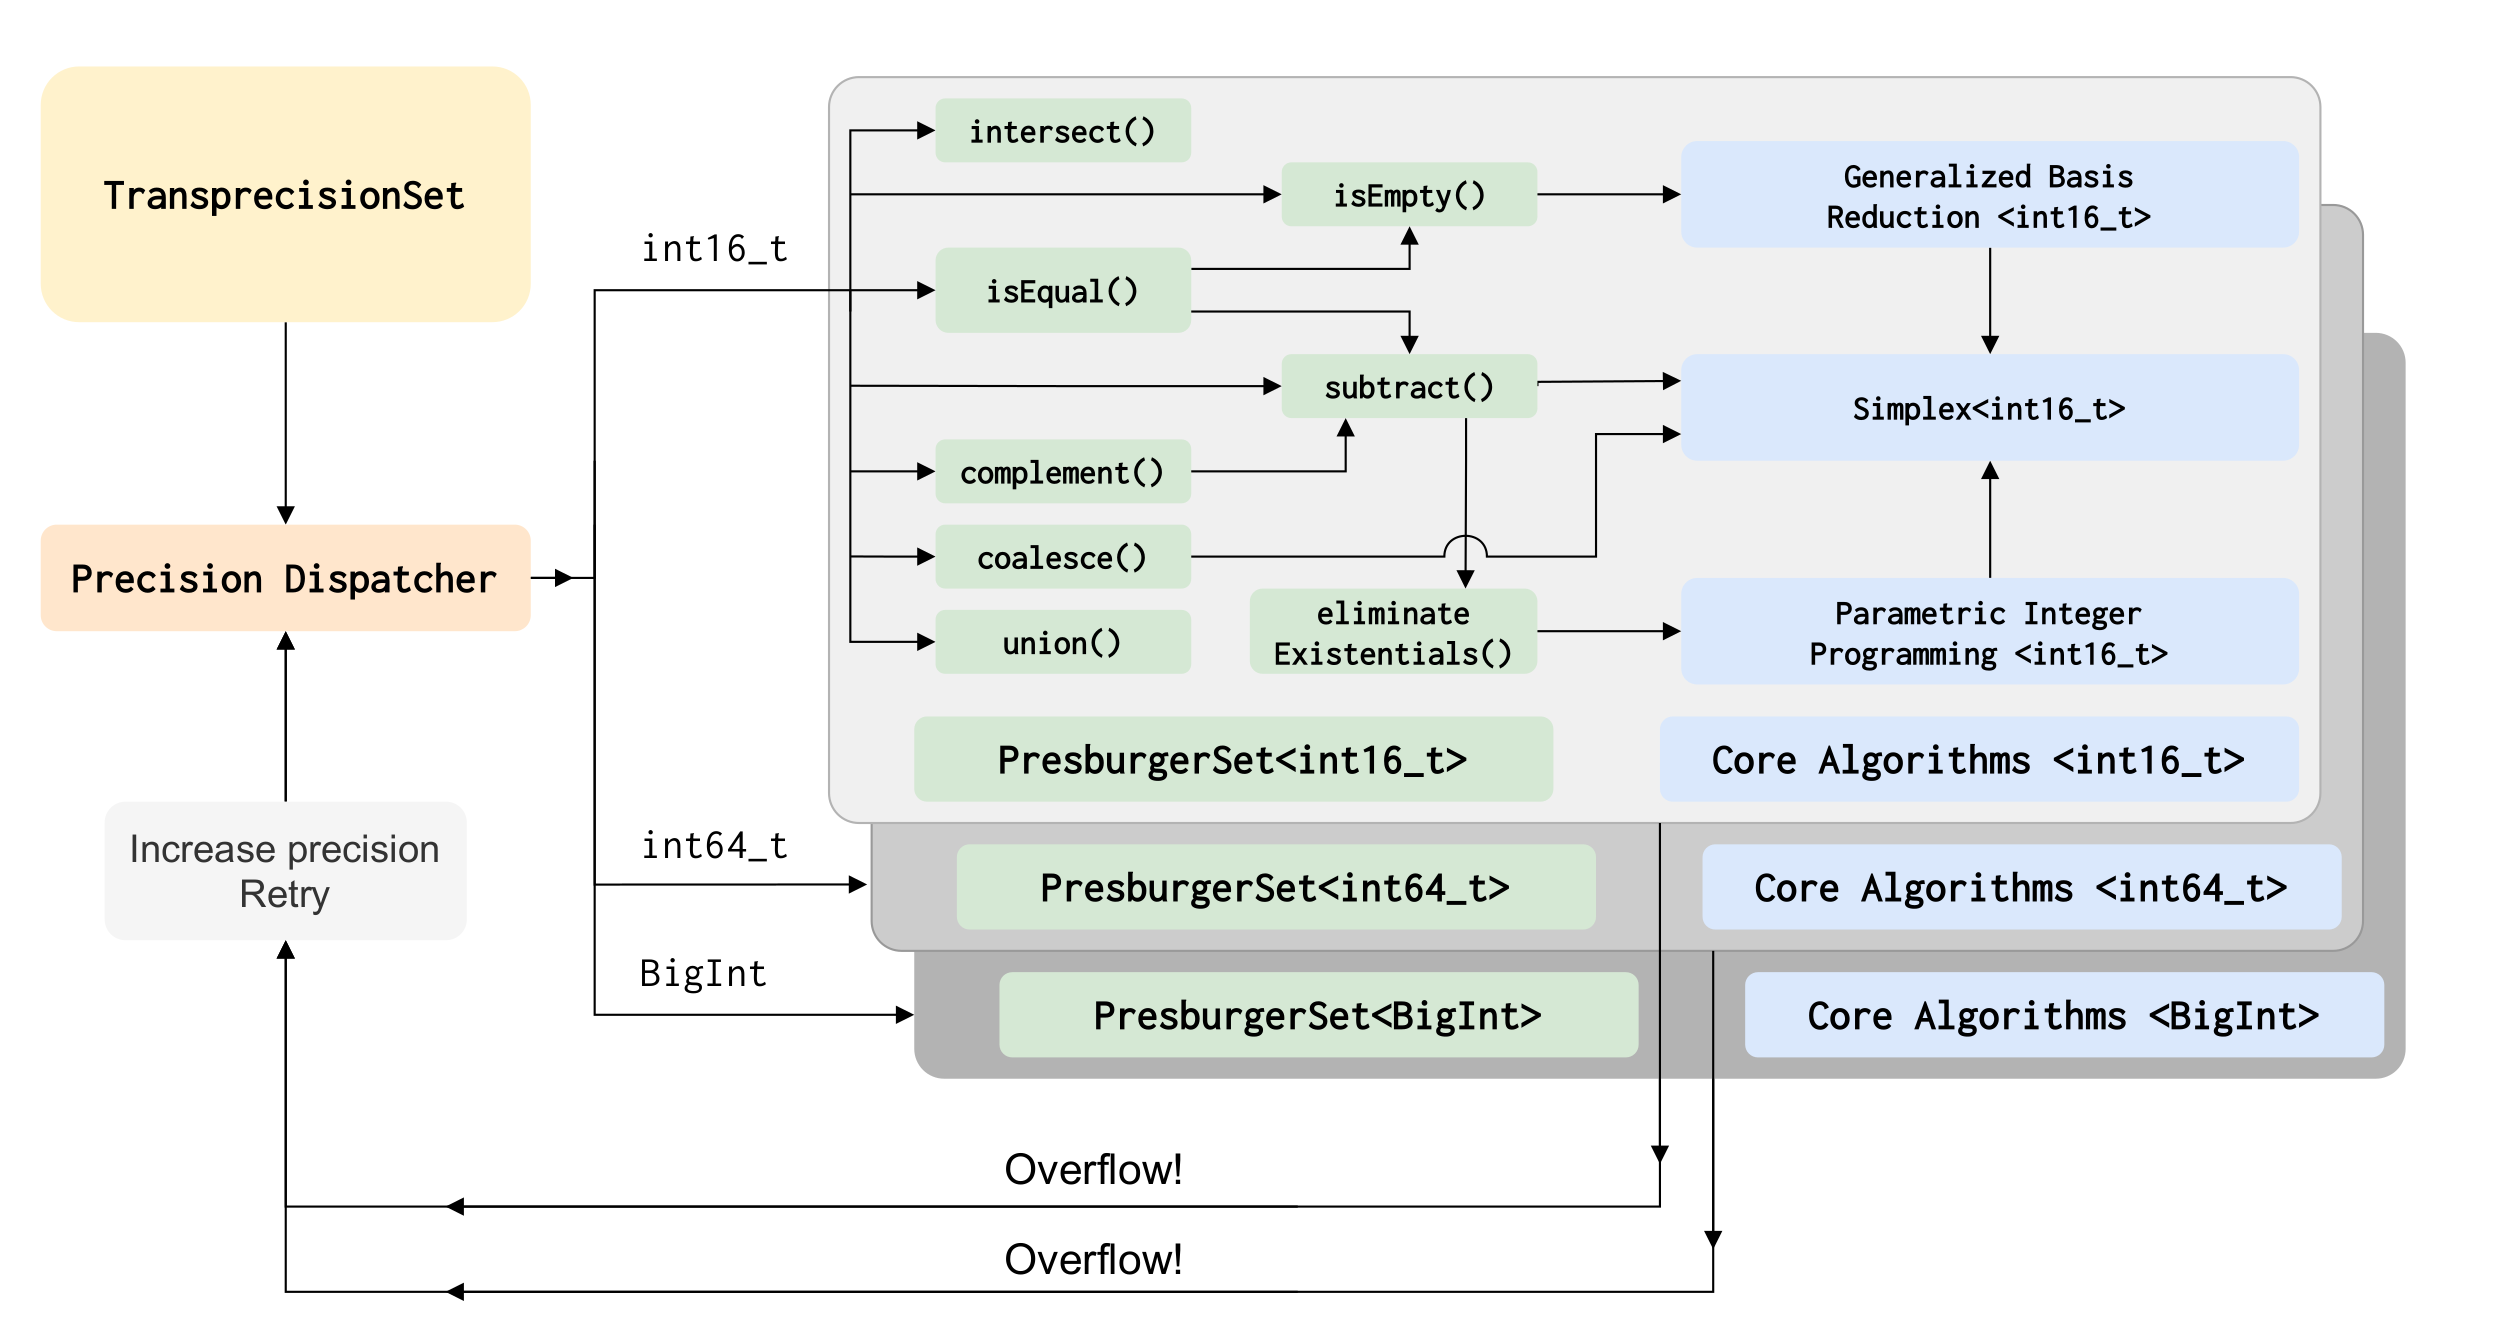
\includegraphics[width=\linewidth]{image/transprecision.png}
    \caption{The The architecture of FPL.}
    \label{fig:fpl_arch}
\end{figure}


\section{Modern CPU micro-architecture}
\label{sec:avx512}

A recent trend in x86-64 architecture’s development is to include AVX-512
instruction set architecture (ISA) extension. AVX-512 succeeds AVX2, the vector
width is increased from AVX-2’s 256 bits to 512 bits. AVX-512 also provides new
instructions, for example, \texttt{int16\_t} saturated addition.

% \subsection{History}

Even though its specification was released by Intel in 2013, it had been
unpopular, as it did not bring practical performance improvements. The primary
reason was that it consumed a lot more power than usual, causing severe
overheating. The micro-architecture Skylake from Intel, and its AVX-512 enabled
counterpart Skylake-X is a classic example. Skylake provides 2 256 bits FMA
AVX-2 execution units 
\footnote{Fused-multiply-add (FMA) execution units are a type of
floating point execution units, capable of doing addition, multiplication or
both in a single instruction. See Section \ref{sec:FMA}.} 
and Intel provides 2 512-bit AVX-512 FMA units by
fusing the existing AVX-2 units into a AVX-512 unit, then introduces an
additional FMA AVX-512 unit \cite{SLK-X}. The additional AVX-512 unit increases
the heat flux density of the chip, causing server thermal throttling issues. 

Intel attempted to mitigate this problem by introducing the ``AVX-offset'' mode.
When a workload involving AVX-512 instructions is encountered, the CPU
automatically enters AVX-offset mode and reduces its clock frequency
\cite{AVX-offset}. However, in practice it is more common to have a mix of
control flow, SSE and AVX-512 instructions, causing many scenario could run
faster if the additional AVX-512 is disabled (and does not thermal throttle)
\cite{Zen4Critique}.

AMD’s implementation of AVX-512 in Zen4 has slightly less computing power, but
much more efficient. Zen4 can be considered as modernized version of Zen3 or
Zen2, where Zen2 and Zen3 supports AVX2 by providing 2 FADD units
\footnote{Floating-point add units (FADD) can to do addition only. They may be 
considered as simplified FMA} 
and 2 FMA units of 256-bit width.
Zen4 merges these existing circuits to create a single 512-bit FADD
and single
512-bit FMA, without introducing any new execution units. Zen3 is reputable for
its high performance per watt (evidence: my experience), and it is expected to
be better on zen4 with more advanced lithography. Benchmarks indicate that this
design indeed does not cause throttling in AVX-512 workloads.
% (https://www.anandtech.com/show/14514/examining-intels-ice-lake-microarchitecture-and-sunny-cove/12#:~:text=2%20%2B%201-,AVX%2D512,-%2D)
% This indicates that it is worthwhile to add software support to AVX-512 and
% gain actual performance increments. 

% Another benefit of AVX-512 is that it reduces front-end pressure. In the case
% of Zen4 microarchitecture, though the back-end is possible to sustain 2 x
% AVX-2 FADD and 2 x AVX-2 FMA every cycle, the front-end has to dispatch 4
% instructions per cycle, which is quite difficult. With AVX-512 it only
% requires 2 instructions to saturate the backend, this is more likely to be
% achievable in a real-world workload.
% (https://www.mersenneforum.org/showthread.php?p=614191)


\section{``\texttt{int23\_t}''}
\label{sec:i23}
\subsection{Fused-multiply-add}
\label{sec:FMA}

\section{code block example}
\begin{verbatim}
    \begin{preliminary}
        ...
    \end{preliminary}
\end{verbatim}

\section{xx}

Computer architecture textbooks often deceipts 

\section{Citations}

Citations (such as \cite{P1} or \cite{P2}) can be generated using
\texttt{BibTeX}. For more advanced usage, we recommend using the \texttt{natbib}
package or the newer \texttt{biblatex} system.

These examples use a numerical citation style. You may use any consistent
reference style that you prefer, including ``(Author, Year)'' citations.

\chapter{Your next chapter}

A dissertation usually contains several chapters.

\chapter{Conclusions}

\section{Final Reminder}

The body of your dissertation, before the references and any appendices,
\emph{must} finish by page~40. The introduction, after preliminary material,
should have started on page~1.

You may not change the dissertation format (e.g., reduce the font size, change
the margins, or reduce the line spacing from the default single spacing). Be
careful if you copy-paste packages into your document preamble from elsewhere.
Some \LaTeX{} packages, such as \texttt{fullpage} or \texttt{savetrees}, change
the margins of your document. Do not include them!

Over-length or incorrectly-formatted dissertations will not be accepted and you
would have to modify your dissertation and resubmit. You cannot assume we will
check your submission before the final deadline and if it requires resubmission
after the deadline to conform to the page and style requirements you will be
subject to the usual late penalties based on your final submission time.

\bibliographystyle{plain}
\bibliography{mybibfile}


% You may delete everything from \appendix up to \end{document} if you don't need it.
\appendix

\chapter{First appendix}

\section{First section}

Any appendices, including any required ethics information, should be included
after the references.

Markers do not have to consider appendices. Make sure that your contributions
are made clear in the main body of the dissertation (within the page limit).

\chapter{Participants' information sheet}

If you had human participants, include key information that they were given in
an appendix, and point to it from the ethics declaration.

\chapter{Participants' consent form}

If you had human participants, include information about how consent was
gathered in an appendix, and point to it from the ethics declaration.
This information is often a copy of a consent form.


\end{document}
